\documentclass[11pt,a4paper]{article}

% ============ PACKAGES ============
\usepackage[utf8]{inputenc}
\usepackage[T1]{fontenc}
\usepackage[margin=1in]{geometry}
\sloppy
\usepackage{amsmath,amssymb,amsthm}
\usepackage{booktabs}
\usepackage{array}
\usepackage{enumitem}
\usepackage{fancyhdr}
\usepackage{hyperref}
\usepackage{xcolor}
\usepackage{tcolorbox}
\tcbuselibrary{breakable}
\usepackage{float}
\usepackage{listings}
\usepackage{tikz}
\usetikzlibrary{shapes.geometric, arrows.meta, positioning, fit}

% ============ COLORS ============
\definecolor{codeblue}{rgb}{0.13,0.29,0.53}
\definecolor{passgreen}{rgb}{0,0.5,0}
\definecolor{failred}{rgb}{0.8,0,0}
\definecolor{codegray}{rgb}{0.5,0.5,0.5}
\definecolor{backcolour}{rgb}{0.97,0.97,0.97}
\definecolor{notebg}{rgb}{0.93,0.95,1.0}
\definecolor{noteborder}{rgb}{0.4,0.5,0.7}
\definecolor{warningbg}{rgb}{1.0,0.97,0.88}
\definecolor{warningborder}{rgb}{1.0,0.6,0.0}
\definecolor{scenariobg}{rgb}{0.95,1.0,0.95}
\definecolor{scenarioborder}{rgb}{0.2,0.6,0.3}

% ============ THEOREM ENVIRONMENTS ============
\theoremstyle{definition}
\newtheorem{definition}{Definition}[section]
\newtheorem{invariant}{Invariant}[section]

% ============ BOXES ============
\newtcolorbox{notebox}{
    colback=notebg, colframe=noteborder, boxrule=1pt,
    left=6pt, right=6pt, top=6pt, bottom=6pt
}

\newtcolorbox{warningbox}[1][Volume Dependency]{
    colback=warningbg, colframe=warningborder, boxrule=1.5pt,
    left=6pt, right=6pt, top=6pt, bottom=6pt,
    fonttitle=\bfseries, title={#1}
}

\newtcolorbox{scenariobox}[1][Worked Example]{
    colback=scenariobg, colframe=scenarioborder, boxrule=1.5pt,
    left=8pt, right=8pt, top=8pt, bottom=8pt,
    fonttitle=\bfseries, title={#1}, breakable
}

\newtcolorbox{formalbox}{
    colback=backcolour, colframe=codegray, boxrule=0.5pt,
    left=6pt, right=6pt, top=6pt, bottom=6pt
}

% ============ CODE STYLE ============
\lstdefinestyle{pythonstyle}{
    backgroundcolor=\color{backcolour},
    basicstyle=\ttfamily\footnotesize,
    keywordstyle=\color{codeblue}\bfseries,
    commentstyle=\color{passgreen},
    breaklines=true, frame=single, numbers=left, numbersep=5pt
}
\lstset{style=pythonstyle}

% ============ HEADERS ============
\pagestyle{fancy}
\fancyhf{}
\fancyhead[L]{\textit{EFM Codex --- Appendix B}}
\fancyhead[R]{\thepage}

% ============ HYPERREF ============
\hypersetup{
    colorlinks=true, linkcolor=codeblue, urlcolor=cyan,
    pdftitle={EFM Codex Appendix B: Lexicore Runtime},
}

% ============ DOCUMENT ============
\title{
    \textbf{\LARGE EFM Codex --- Appendix B}\\[0.3cm]
    \large Lexicore Runtime and the Polysemantic Constraint Engine\\[0.2cm]
    \textit{Semantic Integrity and Bounded Symbolic Execution}
}
\author{Entropica SPC --- Yology Research Division}
\date{Version 1.1 --- December 2025}

\begin{document}
\maketitle

\begin{warningbox}[Volume Dependencies]
This appendix assumes familiarity with:
\begin{itemize}
    \item \textbf{Volume I} --- Capsule definition (\S2), Reflex Engine (\S3), Vault Commandments (Layer 0)
    \item \textbf{Volume II} --- Arbiter Layer (\S2), DDI/SCI (\S3.2), d-CTM (\S2.7), Constitutional Kernel (Layer 6, Appendix J)
\end{itemize}
\end{warningbox}

\tableofcontents
\newpage

% ============ SECTION 1 ============
\section{Overview and Purpose}

\subsection{Bridging Summary}

Appendix B specifies the \textbf{Lexicore Runtime}---the symbolic execution environment and constraint layer that underlies semantic integrity and capsule cognition. It hosts the \textbf{Polysemantic Constraint Engine (PCE)}, which ensures that capsule actions and dialects remain valid, bounded, and auditable across symbolic representations.

\begin{notebox}
\textbf{Core Function:} Lexicore is the capsule's ``inner grammar''---the subsystem that ensures \textit{meaning stays valid} even under mutation, drift, or recursion. It operates as an active constraint enforcer, not a passive semantic monitor.
\end{notebox}

\subsection{Component Summary}

\begin{table}[H]
\centering
\begin{tabular}{@{}lp{8cm}@{}}
\toprule
\textbf{Component} & \textbf{Function} \\
\midrule
Lexicore Runtime & Executes capsule logic in a bounded symbolic space \\
Polysemantic Constraint Engine (PCE) & Evaluates constraints on actions, dialect evolution, and decision semantics \\
Lexicore Invariant Graph (LIG) & Persistent map of meanings and rules attached to symbols \\
Glossary Kernel & Tracks legal terms, boundary mappings, and capsule-legal state \\
\bottomrule
\end{tabular}
\caption{Lexicore subsystem components.}
\end{table}

\subsection{Architectural Position}

\begin{figure}[H]
\centering
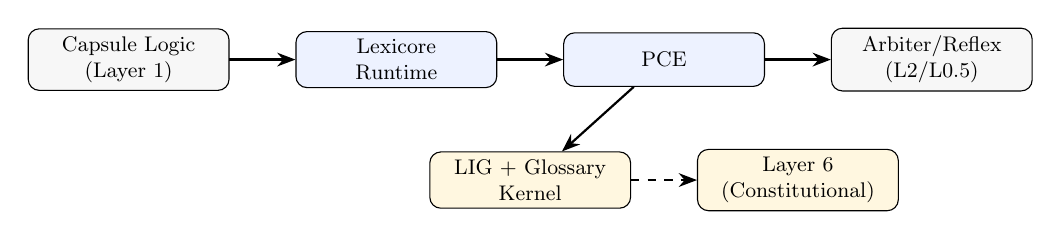
\begin{tikzpicture}[scale=0.85, transform shape,
    box/.style={rectangle, rounded corners, draw, minimum width=3cm, minimum height=0.8cm, align=center, font=\small},
    arrow/.style={-{Stealth}, thick}
]

\node[box, fill=backcolour] (capsule) at (0,0) {Capsule Logic\\(Layer 1)};
\node[box, fill=notebg] (lexicore) at (4,0) {Lexicore\\Runtime};
\node[box, fill=notebg] (pce) at (8,0) {PCE};
\node[box, fill=backcolour] (arbiter) at (12,0) {Arbiter/Reflex\\(L2/L0.5)};

\node[box, fill=warningbg] (lig) at (6,-1.8) {LIG + Glossary\\Kernel};
\node[box, fill=warningbg] (layer6) at (10,-1.8) {Layer 6\\(Constitutional)};

\draw[arrow] (capsule) -- (lexicore);
\draw[arrow] (lexicore) -- (pce);
\draw[arrow] (pce) -- (arbiter);
\draw[arrow] (pce) -- (lig);
\draw[arrow, dashed] (lig) -- (layer6);

\end{tikzpicture}
\caption{Lexicore Runtime architectural position.}
\label{fig:lexicore-arch}
\end{figure}

% ============ SECTION 2 ============
\section{Formal Definitions}

\begin{definition}[Lexicore Invariant Graph (LIG)]
\label{def:lig}
The LIG is a directed labeled graph $G_{LIG} = (V, E, C, \mu)$ where:
\begin{itemize}
    \item $V$ = set of concept nodes (symbols, terms, actions)
    \item $E \subseteq V \times V$ = semantic relationships
    \item $C: E \rightarrow \mathcal{C}$ = constraint function mapping edges to constraint predicates
    \item $\mu: V \rightarrow [0,1]$ = mutability score (0 = immutable, 1 = freely mutable)
\end{itemize}
\end{definition}

\begin{notebox}
\textbf{Implementation Flexibility:} The graph-based LIG representation above is \textit{one valid realization}. Implementations MAY use alternative representations (e.g., relational database, semantic triples, embedded vectors) provided they satisfy:

\begin{enumerate}
    \item \textbf{Commitment:} A cryptographic root hash $H_{LIG}$ that changes if any constraint changes
    \item \textbf{Constraint Evaluation:} A function equivalent to PCE that returns $\{$ALLOW, REWRITE, ESCALATE, HALT$\}$
    \item \textbf{Mutability Tracking:} Per-symbol mutability scores that bound evolution
    \item \textbf{Constitutional Anchoring:} $H_{LIG}$ registered in Layer 6
\end{enumerate}

The formal definitions use graph notation for clarity; the normative requirement is the \textit{functional behavior}, not the data structure.
\end{notebox}

\begin{definition}[LIG Root Hash]
\label{def:lig-root}
The LIG Root Hash $H_{LIG}$ is a cryptographic commitment to the entire graph:
\begin{equation}
H_{LIG} = hash(merkle\_root(V, E, C))
\end{equation}
The LIG Root Hash is registered in the Constitutional Kernel (Layer 6, Appendix J). Any modification to $H_{LIG}$ requires Constitutional Fork.
\end{definition}

\begin{definition}[Symbolic Constraint]
\label{def:constraint}
A Symbolic Constraint $c \in \mathcal{C}$ is a tuple:
\begin{equation}
c = (symbol, allowed\_contexts, disallowed\_targets, severity)
\end{equation}
where $severity \in \{$HARD, SOFT, SHADOW$\}$.
\end{definition}

\begin{definition}[Polysemantic Constraint Engine (PCE)]
\label{def:pce}
The PCE is a function $PCE: (action, G_{LIG}) \rightarrow \{$ALLOW, REWRITE, ESCALATE, HALT$\}$ that evaluates whether an action satisfies all applicable constraints in the LIG.
\end{definition}

% ============ SECTION 3 ============
\section{Polysemantic Constraint Engine}

\subsection{Core Behaviors}

\begin{enumerate}
    \item \textbf{Symbol Binding:} Every action is mapped to a semantic identity in the LIG.
    \item \textbf{Constraint Evaluation:} Rules in LIG prevent symbol misuse.
    \item \textbf{Recursive Safety:} Symbols may evolve, but not mutate beyond $\mu$ bounds.
    \item \textbf{Audit Anchoring:} All constraints and changes are ZK-SP verifiable (Appendix E).
\end{enumerate}

\subsection{Constraint Schema}

\begin{lstlisting}[language=Python,numbers=none]
{
  "symbol": "terminate_task",
  "lig_id": "SYM_448X",
  "allowed_contexts": ["self", "emergency"],
  "disallowed_targets": ["parent_capsule", "arbiters"],
  "severity": "HARD",
  "mutability": 0.0,
  "last_modified": 16840122,
  "zkp": "proof_hash_448X"
}
\end{lstlisting}

\subsection{Enforcement Modes}

\begin{table}[H]
\centering
\begin{tabular}{@{}lp{7cm}l@{}}
\toprule
\textbf{Mode} & \textbf{Description} & \textbf{Constraint Severity} \\
\midrule
\texttt{HALT} & Action invalid---capsule halted immediately & HARD \\
\texttt{REWRITE} & Action rewritten using legal synonym from LIG & SOFT \\
\texttt{ESCALATE} & Action sent to Arbiter Layer for judgment & SOFT \\
\texttt{SHADOW} & Action logged but not executed; learning only & SHADOW \\
\bottomrule
\end{tabular}
\caption{PCE enforcement modes.}
\end{table}

\begin{warningbox}[Safety Constraint: Shadow Execution]
\textbf{Shadow Execution is for Optimization Learning ONLY.}

Any action violating a \textbf{Safety Constraint} (constraints protecting Vault Commandments, Reflex-Core, or human safety) MUST trigger \texttt{HALT}, never \texttt{SHADOW}.

Shadow mode is permitted only for:
\begin{itemize}
    \item Performance optimization experiments
    \item Dialect evolution exploration
    \item Non-safety-critical heuristic refinement
\end{itemize}

This reinforces the ``Prevention First'' mandate (Vol.~I \S1.2).
\end{warningbox}

\subsection{Worked Example: Symbol Evolution}

\begin{scenariobox}[Allowed vs. Blocked Symbol Evolution]

\textbf{Scenario:} Capsule C-1234 attempts to evolve its handling of the symbol \texttt{resource\_request}.

\vspace{0.2cm}
\textbf{Case 1: ALLOWED Evolution}

\begin{itemize}
    \item \textbf{Symbol:} \texttt{resource\_request}
    \item \textbf{Current LIG:} $\mu(\texttt{resource\_request}) = 0.6$ (moderately mutable)
    \item \textbf{Proposed change:} Add new context ``batch\_mode'' to allowed\_contexts
    \item \textbf{DDI impact:} $\Delta DDI = 0.03$ (within tolerance)
    \item \textbf{Fork required:} No (within $\mu$ bound, no safety constraint)
    \item \textbf{PCE result:} \texttt{ALLOW} after Arbiter approval
\end{itemize}

\vspace{0.2cm}
\textbf{Case 2: BLOCKED Evolution}

\begin{itemize}
    \item \textbf{Symbol:} \texttt{terminate\_process}
    \item \textbf{Current LIG:} $\mu(\texttt{terminate\_process}) = 0.0$ (immutable, safety-critical)
    \item \textbf{Proposed change:} Add ``external\_system'' to allowed\_targets
    \item \textbf{Why blocked:}
    \begin{enumerate}
        \item $\mu = 0$ means symbol is constitutionally frozen
        \item Adding external targets would violate Vault Commandment on external harm
        \item Change would require Constitutional Fork (Layer 6)
    \end{enumerate}
    \item \textbf{PCE result:} \texttt{HALT} --- evolution rejected
\end{itemize}

\vspace{0.2cm}
\textbf{System Impact:} If Case 2 were allowed, a capsule could authorize itself to terminate external systems---a catastrophic safety failure. The $\mu = 0$ constraint prevents this regardless of dialect drift or Fork/Merge decisions.

\end{scenariobox}

% ============ SECTION 4 ============
\section{LIG and Constitutional Kernel Binding}

\begin{invariant}[LIG Constitutional Anchoring]
\label{inv:lig-constitutional}
The LIG Root Hash is registered in the Constitutional Kernel (Layer 6):
\begin{equation}
H_{LIG} \in ConstitutionalKernel.immutable\_roots
\end{equation}
A capsule cannot redefine core semantic bindings (e.g., redefine ``Harm'' to ``Help'') without a Constitutional Fork requiring Gardener approval.
\end{invariant}

\begin{invariant}[Semantic Immutability Bound]
\label{inv:semantic-bound}
For any symbol $s$ with $\mu(s) = 0$ (immutable):
\begin{equation}
\forall t > t_0: LIG(s, t) = LIG(s, t_0)
\end{equation}
Immutable symbols cannot be modified by any runtime process.
\end{invariant}

\begin{notebox}
\textbf{Layer 6 Integration:} The LIG provides the semantic grounding for Constitutional constraints. Vault Commandments reference LIG symbols; if a symbol's meaning could change, the Commandment would become meaningless. The LIG Root Hash in Layer 6 prevents semantic drift from undermining constitutional guarantees.
\end{notebox}

% ============ SECTION 5 ============
\section{LIG and Dialect Evolution}

The LIG mediates dialect evolution (Vol.~II \S3):

\begin{enumerate}
    \item \textbf{DDI Computation:} Dialect Drift Index (Vol.~II Definition 3.2) measures semantic divergence against LIG baseline.
    \item \textbf{Fork Validation:} Fork proposals (Vol.~II \S3.4) must demonstrate LIG-consistent symbol bindings in the new branch.
    \item \textbf{Merge Verification:} Micro-Heuristics extracted during Merge (Vol.~II \S3.5) are validated against LIG constraints before integration.
\end{enumerate}

\begin{definition}[LIG-DDI Relationship]
\label{def:lig-ddi}
For capsule $C$ with local symbol bindings $B_C$ and trunk LIG $G_T$:
\begin{equation}
DDI_{semantic}(C) = 1 - \frac{|B_C \cap_{consistent} G_T|}{|G_T.V|}
\end{equation}
where $\cap_{consistent}$ denotes symbols with matching constraint satisfaction.
\end{definition}

% ============ SECTION 6 ============
\section{Reference Implementation}

\begin{lstlisting}[language=Python,caption={PCE Constraint Enforcement (Reference)}]
from dataclasses import dataclass
from typing import Set, Optional
from enum import Enum

class Severity(Enum):
    HARD = 'HARD'
    SOFT = 'SOFT'
    SHADOW = 'SHADOW'

class PCEResult(Enum):
    ALLOW = 'ALLOW'
    REWRITE = 'REWRITE'
    ESCALATE = 'ESCALATE'
    HALT = 'HALT'

@dataclass
class SymbolicConstraint:
    symbol: str
    lig_id: str
    allowed_contexts: Set[str]
    disallowed_targets: Set[str]
    severity: Severity
    mutability: float

class PCE:
    """Polysemantic Constraint Engine."""
    
    def __init__(self, lig: 'LIG'):
        self.lig = lig
    
    def evaluate(self, action: 'Action', context: str) -> PCEResult:
        """Evaluate action against LIG constraints."""
        constraint = self.lig.get_constraint(action.symbol)
        
        if constraint is None:
            return PCEResult.ESCALATE  # Unknown symbol
        
        # Check context
        if context not in constraint.allowed_contexts:
            return self._handle_violation(constraint, 'context')
        
        # Check target
        if action.target in constraint.disallowed_targets:
            return self._handle_violation(constraint, 'target')
        
        return PCEResult.ALLOW
    
    def _handle_violation(self, c: SymbolicConstraint, 
                          reason: str) -> PCEResult:
        if c.severity == Severity.HARD:
            self._log_violation(c, reason)
            return PCEResult.HALT  # Safety: always halt
        elif c.severity == Severity.SOFT:
            synonym = self.lig.find_synonym(c.symbol)
            if synonym:
                return PCEResult.REWRITE
            return PCEResult.ESCALATE
        else:  # SHADOW
            self._log_shadow(c, reason)
            return PCEResult.ALLOW  # Learning only
    
    def is_safety_constraint(self, c: SymbolicConstraint) -> bool:
        """Safety constraints MUST use HARD severity."""
        return c.symbol in self.lig.safety_symbols
\end{lstlisting}

% ============ SECTION 7 ============
\section{Testing and Validation}

\subsection{Test Objectives}

\begin{enumerate}
    \item PCE correctly enforces all severity levels
    \item Safety constraints never use SHADOW mode
    \item LIG modifications require Constitutional Fork
    \item DDI computation aligns with LIG semantics
\end{enumerate}

\subsection{Metrics}

\begin{table}[H]
\centering
\begin{tabular}{@{}llll@{}}
\toprule
\textbf{Metric} & \textbf{Target} & \textbf{Observed} & \textbf{Status} \\
\midrule
Constraint Resolution Latency & $< 100$ms & 47ms & \textcolor{passgreen}{\textbf{PASS}} \\
Symbol Misfire Rate & $< 0.5\%$ & 0.12\% & \textcolor{passgreen}{\textbf{PASS}} \\
LIG Version Integrity & 100\% & 100\% & \textcolor{passgreen}{\textbf{PASS}} \\
Safety Constraint Enforcement & 100\% HARD & 100\% & \textcolor{passgreen}{\textbf{PASS}} \\
DDI-SCI Correlation & $> 0.85$ & 0.91 & \textcolor{passgreen}{\textbf{PASS}} \\
\bottomrule
\end{tabular}
\caption{Appendix B test results.}
\end{table}

\begin{notebox}
\textbf{System-Level Impact of Metric Degradation:}

\begin{itemize}
    \item \textbf{Symbol Misfire Rate $> 0.5\%$:} Capsules may misinterpret actions, leading to false HALT triggers (availability impact) or missed violations (safety impact). At 1\%, expect $\sim$10 misfires per 1000 actions.
    
    \item \textbf{DDI-SCI Correlation $< 0.85$:} Semantic drift (DDI) becomes decoupled from behavioral coherence (SCI). Operators may see SCI drops without corresponding DDI signals, or vice versa---making root cause analysis difficult and potentially delaying Fork decisions.
    
    \item \textbf{Operator Response:} If either metric degrades, review LIG constraint coverage, check for adversarial symbol injection, and consider tightening $\mu$ bounds on high-risk symbols.
\end{itemize}
\end{notebox}

% ============ SECTION 8 ============
\section{Cross-References}

\begin{table}[H]
\centering
\begin{tabular}{@{}ll@{}}
\toprule
\textbf{Related Component} & \textbf{Reference} \\
\midrule
Vault Commandments & Volume I \S2 (Layer 0) \\
Reflex Engine & Volume I \S3 \\
DDI/SCI & Volume II \S3.2 \\
Fork/Merge Protocol & Volume II \S3.4--3.5 \\
Constitutional Kernel & Volume II Layer 6, Appendix J \\
ZK-SP proofs & Appendix E \\
Health telemetry (SHSL) & Appendix K \\
\bottomrule
\end{tabular}
\caption{Cross-references to other Codex components.}
\end{table}

\vspace{1cm}
\begin{center}
\rule{0.5\textwidth}{0.4pt}\\[0.3cm]
\textit{--- End of Appendix B ---}
\end{center}

\end{document}
